\documentclass{article}
\usepackage[utf8]{inputenc}
\usepackage{geometry}
\usepackage{graphicx}
\usepackage{lipsum}
\usepackage{enumitem}
\usepackage{amssymb}
\usepackage{adjustbox}
\usepackage{hyperref}
\usepackage{breakurl}
\usepackage{amsmath}
\usepackage{ulem}
\usepackage{float}
\usepackage{subcaption}
\usepackage{changepage}  % Paquete para ajustar márgenes
\usepackage{booktabs} % Para líneas horizontales en tablas
\usepackage[table]{xcolor}
\usepackage{pgfplots} % Para gráficos
\pgfplotsset{compat=1.18}
\usepackage{url}
\usepackage{afterpage}
\usepackage{titlesec}


\titleclass{\subsubsubsection}{straight}[\subsubsection]
\newcounter{subsubsubsection}[subsubsection]
\renewcommand\thesubsubsubsection{\thesubsubsection.\arabic{subsubsubsection}}
\titleformat{\subsubsubsection}
  {\normalfont\normalsize\bfseries}{\thesubsubsubsection}{1em}{}
\titlespacing*{\subsubsubsection}
  {0pt}{3.25ex plus 1ex minus .2ex}{1.5ex plus .2ex}
  
\geometry{a4paper, margin=1in}

\titleformat{\section}
{\normalfont\Large\bfseries}{\thesection}{1em}{}

\begin{document}
\begin{titlepage}
    \centering
    \vspace*{2cm}
    
    {\Large\textbf{R. P. FRANCISCO SUÁREZ}}\\
    {\large Granadino de la Compañía de Jesús,}\\
    {\large Doctor Eximio,}\\[1.5cm]
    
    {\Huge\textbf{TRATADO TEOLÓGICO,}}\\[0.5cm]
    {\Large\textbf{SOBRE LA VERDADERA INTELIGENCIA DEL AUXILIO EFICAZ,}}\\
    {\large y su Concordancia con el libre albedrío.}\\[0.5cm]
    % Añadir imagen aquí
    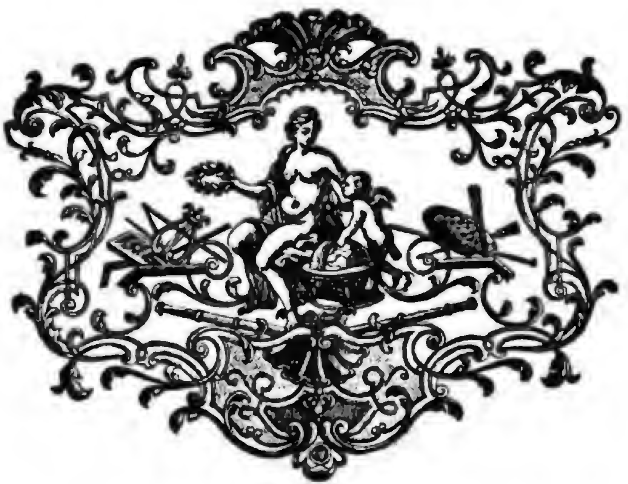
\includegraphics[width=0.4\textwidth]{portada.png}\\[0.5cm]

    
    {\large OBRA PÓSTUMA.}\\[1cm]
    
    {\large Adaptada para establecer las definiciones de la Fe, por nuestro Santo Padre INOCENCIO X,}\\
    {\large contra los jansenistas y sus partidarios.}\\[1.5cm]
    
    {\large NOVENO TOMO DE LAS OBRAS.}\\[1.5cm]
    
    {\Large\textbf{VENECIA,}}\\
    {\large De la Tipografía Balleoniana.}\\[0.5cm]
    {\large 1741.}\\[0.5cm]
    
    {\large Con permiso y privilegios de los Superiores.}
    
    \vfill
\end{titlepage}

\begin{center}
    \textbf{PEQUEÑA ADVERTENCIA AL LECTOR}
\end{center}
HAY DOS COSAS que deben mencionarse brevemente en este prólogo: EL AUTOR Y EL LIBRO. Sobre ambos, es importante advertir al lector, y a mí me conviene no callar por completo.

Pero sobre el Autor, parecerá que he hablado suficiente y en exceso si digo que él es FRANCISCO SUÁREZ, el singular ornamento de su época y el astro más brillante de la Escuela Teológica. Las obras que él mismo ha realizado dan testimonio de ello. ¿Qué tan grande fue el vientre de su ingenio, del cual surgió una cosecha tan abundante y noble? ¿Cuál fue esa fábrica de doctrina, de donde salió una riqueza casi inmensa para la Teología, y un remedio muy eficaz contra el veneno mortal de la ignorancia, preparado para el gran bien de la Iglesia? Hasta ahora han visto la luz, por obra de SUÁREZ, más de veintidós voluminosos tomos sobre casi todos los argumentos teológicos y filosóficos. Queda por publicar uno o dos tomos sobre los Consejos y respuestas a varias cuestiones, y sobre lógica y otros temas relacionados con las cuestiones de Aristóteles: Si añades estos a los VEINTICINCO tomos que ahora presentamos, descubriremos que la obra literaria ha sido enriquecida por él. Con razón he dicho enriquecida. Francisco Suárez no emitió libros como los que muchos producen en esta época de escritura apresurada: verdes, áridos, sin jugo, destinados pronto a servir como envoltura de incienso o pimienta, y como fundas para peces, debido a la falta de sustancia del corazón de sus autores. Las lucubraciones de Suárez son todas maduras, sólidas, fuertes, llenas de buen jugo, nutridas de erudición, y recomendadas por la prerrogativa de un juicio y método eximios. Así que Alfonso de Castelbranco, el Ilustrísimo Obispo de Coímbra, no dudó, cuando habló sobre la obra de defensa de la fe, en elogiar universalmente y de manera destacada los escritos de Suárez, llamándolo el MAESTRO UNIVERSAL DE SU ÉPOCA, y refiriéndose a él como el SEGUNDO AGUSTÍN. Tampoco fueron menos generosos en sus elogios otros dos Ilustrísimos y Sapientísimos Prelados: Don Fernando Martínez Mascareñas, Obispo de los Algarvios, más tarde el supremo Inquisidor de la Fe en Lusitania; y Don Martín Alfonso de Melo, Obispo de Lamego. No faltó quien, en el mismo campo de alabanzas a Suárez, lo celebrara. Hubo quien lo llamara el Oráculo de la Sabiduría, quien lo llamara el prodigio de su época, y quien, con un epíteto muy notable, lo denominara el Gigante de la Teología Escolástica. Todo puede parecer resumido en el epitafio mortal, además de otras cosas colocadas en el monumento funerario en sus exequias, donde Suárez es llamado: MAESTRO DE EUROPA Y AUN DE TODO EL MUNDO; ARISTÓTELES EN LAS CIENCIAS NATURALES; TOMÁS DE AQUINO EN LAS DIVINAS; JERÓNIMO EN LA ESCRITURA; AMBROSIO EN LA CÁTEDRA; AGUSTÍN EN LAS POLÉMICAS; ATANASIO EN LA EXPLICACIÓN DE LA FE; BERNARDO EN LA MIELIFLUA PIEDAD; GREGORIO EN EL TRATAMIENTO DE LAS ESCRITURAS; EL OJO DEL PUEBLO CRISTIANO; Pero según su propio juicio, NADA. Me abstengo de decir más, porque entre todos los doctos, Suárez es alguien que no necesita elogios. Y así, la primera tarea que en este prólogo me había propuesto exponer, queda expuesta.

Es necesario referirse al libro que ahora sale a la luz por primera vez, para cumplir con la otra promesa. Que es una obra genuina de Suárez, lo demostrará en primer lugar su lectura, incluso si se hace de manera superficial y rápida. Porque no hay huevo más parecido a otro huevo, ni gota más similar a otra gota, que este escrito con respecto a las otras obras indudables de Suárez. El mismo adorno de juicio, solidez, claridad y método en todas partes. Además, los hombres muy versados en letras, que han tenido la oportunidad de leer esta obra, no admiten que ningún escrito de Suárez sobre este tema se pueda comparar con esta obra. De los muchos y excelentes testigos que tengo a mano, presento uno muy autorizado: Fernando de Bastida, a quien no ignora ningún rincón de España. Que fue un hombre de un ingenio sobresaliente puede ser demostrado por el hecho de que, al percibir su capacidad, aquellos a quienes más les interesaba, en la controversia sobre los auxilios de la gracia divina ante los pontífices Clemente VIII y Paulo V, lo asignaron, aún sin haber recibido la ordenación, como sucesor de Gregorio de Valencia, teólogo incomparable. Tan alta era la opinión sobre él, que no dudaron en confiar un asunto de tanta importancia y lleno de peligrosa incertidumbre a este joven teólogo. Se le escuchó decir a menudo sobre esta lucubración de Suárez que conservaba consigo, que no concedía a ningún otro escrito de Suárez sobre este tema lo que concedía a esta; que se atrevía incluso a afirmar que superaba a todos. Bastida la había traído consigo a España al regresar de Roma. Pues allí mismo, en Roma, había sido escrita por Suárez, para refutar todas las objeciones que había escuchado plantear contra sus escritos anteriores; para reafirmar lo suyo y refutar lo ajeno; y si en sus escritos anteriores algo pareciera necesitar mayor claridad, para ilustrarlo con nuevos rayos de luz. Entonces, Bastida, al regresar a España, se llevó consigo el volumen escrito por Suárez; y mientras vivió, lo conservó como un tesoro precioso, del cual parecía no poder saciarse de elogios. Pero antes de pasar a otras manos, lo confió a un amigo singular, un hombre de doctrina sobresaliente. Este, con buenos augurios, nos lo envió para que se hiciera de dominio público, considerando que, con gran perjuicio para las letras, e incluso para la Iglesia, sería envidiable que una obra tan excelente, cuya utilidad podría ser notable para confirmar lo que nuestro Santo Padre Inocencio X, no hace mucho, había declarado providencialmente contra las cinco herejías de Calvino, provenientes de la insidiosa Batavia, que ciertamente causarían gran daño a la doctrina católica si no se erradicaran. Eso es lo que principalmente busca Suárez en todo este volumen: refutar esas herejías; establecer la gracia suficiente; demostrar los auxilios eficaces y eluctables, y que coherentemente se corresponden con la libertad humana; confirmar sólidamente y con precisión que Cristo murió por todos, en virtud de que, gracias a su beneficio, todos tienen a su alcance la gracia para salvarse si no tienen una mente obstinada; manifestar que los mandamientos divinos, con la misma gracia otorgada a todos, pueden ser observados, contrario a lo que sostenían los tumores jansenistas en torno a la fe, que fueron truncados por la espada apostólica para que no infectaran el cuerpo místico de Cristo, algo que todos los buenos celebran. Así pues, a la Iglesia le ha parecido conveniente, con la publicación de esta obra, confirmar esas cinco definiciones pontificias, contra los pocos que aún murmuran y buscan excusas en los pecados, a través de sentidos distorsionados y oscuridades buscadas en pleno mediodía. De ahí surge la esperanza indudable de que esta lucubración tan oportuna, de un hombre cuyas grandes contribuciones a la Teología y cuyos trabajos exquisitos en favor de la Iglesia de Dios lo recomiendan, será muy bien recibida por todos los que se esfuerzan y aman la doctrina sana en todas partes. Y porque al vino vendible no le hace falta la hiedra, me abstengo de una mayor ornamentación, tanto del Autor como de la Obra.

AL FINAL del volumen, que podría parecer más modesto en tamaño, se ha añadido una defensa no inapropiada de Suárez, en relación con la gracia administrada por un sacerdote presente al enfermo oprimido. Porque algunos, respecto a lo que se había establecido en Roma bajo Paulo V. en relación con la glosa aplicada al decreto de Clemente VIII., lo habían llevado a la censura y condena de la doctrina enseñada por Suárez; más allá, o más bien en contra de la intención expresa del mismo pontífice Paulo, quien quiso que la doctrina de Suárez en ese punto se mantuviera íntegra y sin daño, y que permaneciera en los libros sagrados públicos como ya estaba, o incluso antes, insertada; el veterano y amante de la verdad Suárez, Don Atanasio Solerius, Doctor en Sagrada Teología de Comitatense, sin tocar lo que se había establecido en Roma, emprendió la tarea de disipar la injuria infligida al mejor Maestro por la distorsión del decreto romano, y reprimió al joven Ayax que insultaba a los ancianos; demostrando que lo establecido en Roma tenía otro propósito y no invalidaba la doctrina de Suárez sobre la absolución del moribundo. Pareció oportuno añadir a la obra de Suárez, que ahora damos, esa breve lucubración, traída de regreso a España por un hombre destacado en escritos teológicos, y comunicada oportunamente al mismo tiempo que se envió la defensa de Suárez; debido a la necesidad de los argumentos, ya que ambos escritos tratan sobre la gracia y contienen la defensa del mismo Autor desde diferentes perspectivas. Disfruta, lector, y SALUD.

\newpage
\tableofcontents
\newpage

\begin{center}
    \textbf{TRATADO DEL DOCTOR FRANCISCO SUÁREZ GRANADINO, DE LA COMPAÑÍA DE JESÚS}\\
    ACERCA DE LA VERDADERA INTELIGENCIA DEL AUXILIO EFICAZ Y SU CONCORDANCIA CON LA LIBERTAD DEL CONSENTIMIENTO VOLUNTARIO.
\end{center}

\section{PROOEMIUM.}
Aunque he discutido esta cuestión en un opúsculo sobre la concurrencia y el auxilio eficaz de Dios según mis fuerzas, y he tratado de definirla conforme a la sincera verdad de las Escrituras, y la tradición de los Padres y de los Concilios; sin embargo, la amplitud y la gravedad de la materia nos obligan a añadir algunas cosas a lo anterior. Especialmente porque, con motivo de algunas disputas que se han escrito posteriormente sobre este tema, se nos ha preparado el camino para estabilizar más la verdad allí enseñada y, lo que es fundamental, para explicarla de tal manera que no pueda ser oscurecida por ningún falso título de error. Tan firme e inconmovible es la verdad establecida allí, que no solo no puede ser socavada por los adversarios, sino que tampoco puede ser aparentemente impugnada, excepto inventando varias cosas y atribuyéndonos monstruos de errores, hacia los cuales dirigen sus armas argumentativas. De las cuales no podría no surgir alguna infamia o al menos sospecha de nuestra doctrina entre la gente común, a menos que dejáramos clara y manifiesta la ocasión de engaño tomada, más que dada.

Por lo tanto, no repetiré en este lo que se dijo en el opúsculo anterior; sino que, retomando brevemente el punto de la controversia y la disensión, y explicando ambas opiniones de tal manera que, apartando las cuestiones sobre nombres o el uso de términos, se entienda qué hay de contradicción en la realidad misma, mostraremos en detalle cuán lejos está nuestra sentencia de los errores que se nos atribuyen a nosotros o a otros Doctores de nuestra Compañía. Después examinaremos la fidelidad de todos los testimonios que hemos presentado a nuestro favor, y a los cuales se objeta que han sido alegados infielmente por nosotros o mal interpretados. Finalmente, evaluaremos la fuerza de nuestros argumentos y, con esa ocasión, expondremos la nueva doctrina que los adversarios introducen, y analizaremos cuidadosamente su calidad y todos los testimonios y razones con los que intentan nuevamente confirmar sus dogmas. En esta obra no nos guiamos por un espíritu de contradicción, sino que simplemente buscamos una justa defensa. Tampoco deseamos anticiparnos al juicio de la Sede Apostólica, a la cual siempre nos sometemos; sino que nos vemos obligados a ofrecer una información más completa de toda nuestra sentencia, tanto para evitar que la verdad misma sufra algún inconveniente por la falsa sospecha de algún error o por una interpretación parcial de nuestra mente, como también porque se trata de una cuestión muy grave y extremadamente necesaria en estos tiempos, en la que no se debe permitir ninguna sospecha de error por parte de un Doctor Católico.

\section{CAPUT PRIMUM. Se supone la existencia de la gracia eficaz, y se defiende brevemente la distinción entre gracia eficaz y suficiente.}

Se supone en el título de toda la obra la existencia de la gracia eficaz, que es casi el propósito, o más bien el centro de toda la controversia presente: ya que, al explicar la naturaleza y la eficacia de esa gracia, que no daña el uso de la libertad, se ha establecido todo este asunto. En estos días, un pequeño libro ha salido a la luz, en el cual el autor cree haber refutado agudamente (según él mismo piensa) la distinción entre gracia suficiente y eficaz, y considera que ha eliminado toda ocasión de controversia. Además, opina que ha conciliado fácilmente la libertad con la gracia que excita y ayuda. Sin embargo, apenas se puede entender a partir del discurso de ese autor cuál es su intención o de qué manera finalmente enseña que la libertad se concilia con las predicciones divinas o la predestinación. Ni siquiera se entiende si simplemente desea negar que exista una gracia que sea únicamente suficiente y otra que sea simultáneamente suficiente y eficaz, o si en realidad impugna solo la división de la gracia en esos dos miembros, ya sea porque los miembros no están claramente diferenciados o porque no se ha explicado suficientemente hasta ahora.

Y ciertamente, si se examina el propósito del libro y las palabras con las que se presentan en muchos capítulos desde el principio, parece que se enseña absolutamente que no existe ninguna gracia eficaz, ni siquiera ninguna que sea únicamente suficiente. Pero este sentido no solo es erróneo, sino que también es tan abiertamente contrario a la doctrina del mismo autor, que no es probable que un hombre prudente y no ignorante haya tenido esa intención. Porque es tan cierto que existe una gracia suficiente como lo es que Dios no impide que los hombres se salven. Esto lo dijo plenamente el Sabio en Eclesiástico 15: \textit{No digas: 'Dios está ausente', porque lo que él desea, lo hará}. Y todas las razones con las que el autor impugna la mencionada división en cuanto a este aspecto, en realidad demuestran más bien que existe una gracia verdaderamente suficiente en la realidad misma, y no solo en nombre, lo cual admitimos plenamente. Además, demuestran que tal gracia verdaderamente suficiente no solo se da a los predestinados, sino también a los reprobos, no solo a aquellos que consienten, sino también a aquellos que resisten.

Por lo tanto, queda claramente demostrado que existe una gracia que es únicamente suficiente, es decir, que aunque sea adecuada en sí misma y inmediatamente capaz de producir el efecto, no obstante no alcanza a producir el efecto. Esto es tan evidente, tanto desde el punto de vista del autor como desde los hechos mismos, que probarlo se vuelve innecesario. Si una gracia de este tipo sea suficiente en términos de su capacidad, y no alcance el efecto debido a la falta de una gracia adicional, que no está en el poder del hombre, o por alguna incongruencia pretendida y capturada por Dios, o solamente debido a un defecto del hombre y el abuso de la libertad, es otra cuestión. En este caso, también sentimos que esto no proviene de la falta de una gracia adicional que preceda, la cual no está en el poder del hombre; de hecho, si la gracia previa fuera suficiente en sí misma, no solo en nombre sino en realidad. Tampoco proviene de alguna incongruencia inherente a tal gracia, ya que esta gracia, en su primer acto, ni está atrapada ni pretendida por Dios, quien, al contrario, desea fervientemente que el hombre se convierta y acepte tal gracia. Más bien, decimos que esto proviene únicamente de la libertad innata del hombre, según aquello que dice: \textit{Tu perdición proviene de ti mismo}. De esta libertad resulta que una gracia que podría ser adecuada en sí misma se convierte en incongruente en el segundo acto, es decir, vana, inútil e ineficaz. Por lo tanto, dado que Dios, quien otorga tal gracia, no ignora la incongruencia futura, se dice que otorga una gracia incongruente no en el primer acto ni en sí misma, sino en el segundo acto y debido al hombre, no con la intención de crear incongruencia, sino previendo y permitiendo. Por lo tanto, tal gracia se llama meramente o puramente suficiente. Y dado que ese autor no advirtió la diferencia entre captar la incongruencia o permitirla, y la diferencia entre la inadecuación en el primer acto, o en sí misma, de la inadecuación en el segundo acto, por lo que impugna fríamente este punto de su división como si estuviera correctamente comprendido, aunque bien combate algunas de sus exposiciones que no son en absoluto adecuadas.

En cuanto al otro aspecto del auxilio eficaz, el autor también procede de manera confusa, al distinguir la ambigüedad de esa palabra, como mencioné en otro lugar; lo cual creo que también le ha ocurrido a este autor. Pues eficacia suele significar no la eficiencia actual, ni la capacidad de obrar, que siempre conlleva eficacia en el segundo acto, sino solo la virtud que proporciona verdaderas fuerzas activas, y en cuanto a sí misma, inferir eficacia actual, aunque puedan ser impedidas de otra manera, y se lleguen a impedir. En este sentido, todo auxilio verdaderamente suficiente es también eficaz, es decir, verdaderamente efectivo. También suele significarse por eficacia la sola eficiencia actual, o la virtud, como unida a la eficiencia actual: en cuyo sentido es evidente que no todo auxilio suficiente es eficaz, y se dan muchos auxilios así suficientes, de modo que también son eficaces, es decir, actualmente eficientes: en efecto, siempre que el hombre realiza libremente algún acto sobrenatural, ese acto es el efecto en el que actualmente influye algún auxilio divino: y, por lo tanto, es igualmente cierto que allí interviene el auxilio eficaz en el sentido mencionado. Por ello, el mismo autor, que en un lugar parece negar la gracia eficaz incluso bajo esta denominación, en otro la aprueba, y según la mente de Santo Tomás, dice que se llama gracia eficaz, no por la diferencia de calidad, sino por la misma eficiencia y el acto segundo de la eficacia: ni considera inconveniente que esa denominación de gracia eficaz no sea sin el concurso del libre albedrío, lo cual había impugnado en el lugar anterior.

Por otro lado, la gracia suele llamarse eficaz aquella que promueve la voluntad de tal manera que la hace actuar infaliblemente en lo que Dios intenta: y parece que el autor principalmente impugna esta gracia eficaz, aunque sus razones valen algo contra aquellos que postulan que tal gracia tiene una infalibilidad causal, por así decirlo, es decir, que proviene de la naturaleza de tal auxilio que tiene la fuerza de predeterminar la voluntad a uno y al ejercicio del acto. Sin embargo, valen poco contra aquellos que solo admiten la infalibilidad proveniente, no de la sola eficacia innata del auxilio, sino de la que subyace en la presciencia divina de los condicionados contingentes. Esta presciencia la impugna débilmente, como mostraré en otro lugar: y repite y exagera mucho que de ahí se sigue una inconveniencia de la gracia, que debe ser atribuida a Dios como si buscara ocasiones para perder a los hombres. Lo cual es también frívolo: pues Dios, en virtud de su presciencia, no es causa de los defectos humanos, de modo que estos le puedan ser atribuidos por esa razón: ni tampoco intenciona tales defectos, sino que los permite.

Por lo tanto, suponemos con certeza que existe una gracia preveniente, ya sea excitante o operante, eficaz en esta última significación. Porque sin ella no puede haber elección, predestinación o predeterminación de actos libres, los cuales, en el orden de la razón, preceden la presciencia absoluta de las obras futuras libres. Porque si Dios ha determinado con un Decreto absoluto que Pedro, por ejemplo, tenga aquí y ahora un acto de contrición, antes de prever que Pedro tendría tal acto, es necesario que tenga el poder de mover e inclinar la voluntad de Pedro hacia tal acto, de manera que sea totalmente infalible para Dios que se cumplirá lo que ha decretado; pues de otra manera, la voluntad absoluta de Dios no se cumpliría infaliblemente, lo cual es contrario a la perfección y omnipotencia divina. Ni el autor mencionado en toda esa obra explica cómo, sin esta gracia eficaz, la predestinación divina, explicada de la manera dicha, puede tener certeza e infalibilidad sin la gracia eficaz preveniente.




































































































\end{document}
